\section{Aufbau}
\label{sec:Aufbau}

In Abbildung \ref{fig:aufbau} ist eine schematische Skizze des Aufbaus dargstellt.
Durch eine Rubidiumspektrallampe wird Licht emittiert, welches zunächst kollimiert wird.
Dahinter wird ein Interferenzfilter geschaltet um nur die $D_1$-Wellenlänge durchzulassen.
Im Anschluss wird das Licht linear polarisiert und mittels eines $\lambda/4$-Plättchens
rechtszirkular polarisiert. Danach fällt es auf die Dampfzelle.
Für Licht aus thermischen Emissionen gilt, dass alle Übergänge erlaubt sind,
da es eine gewisse Linienbreite aufweist.

Innerhalb der Dampfzelle befindet sich das Rubidum-Neon Gasgemisch. Der Neonanteil sorgt dafür,
dass es keine Besetzungsinversion gibt wenn die Rubidumatome mit den Wänden der Dampfzelle kollidiert.
Außerdem wird bei Stößen zwischen Neon- und Rubidumatomen kein Drehimpuls zwischen den
Elektronenhüllen ausgetauscht, sodass das herstellen der Besetzungsinversion nicht abgeschwächt wird.
Das Licht wird nach dem hindurchtreten durch die Dampfzelle in eine Photozelle fokussiert, sodass die
Transparenz des Gases für die $D_1$-Linie gemessen werden kann.
\begin{figure}
    \centering
    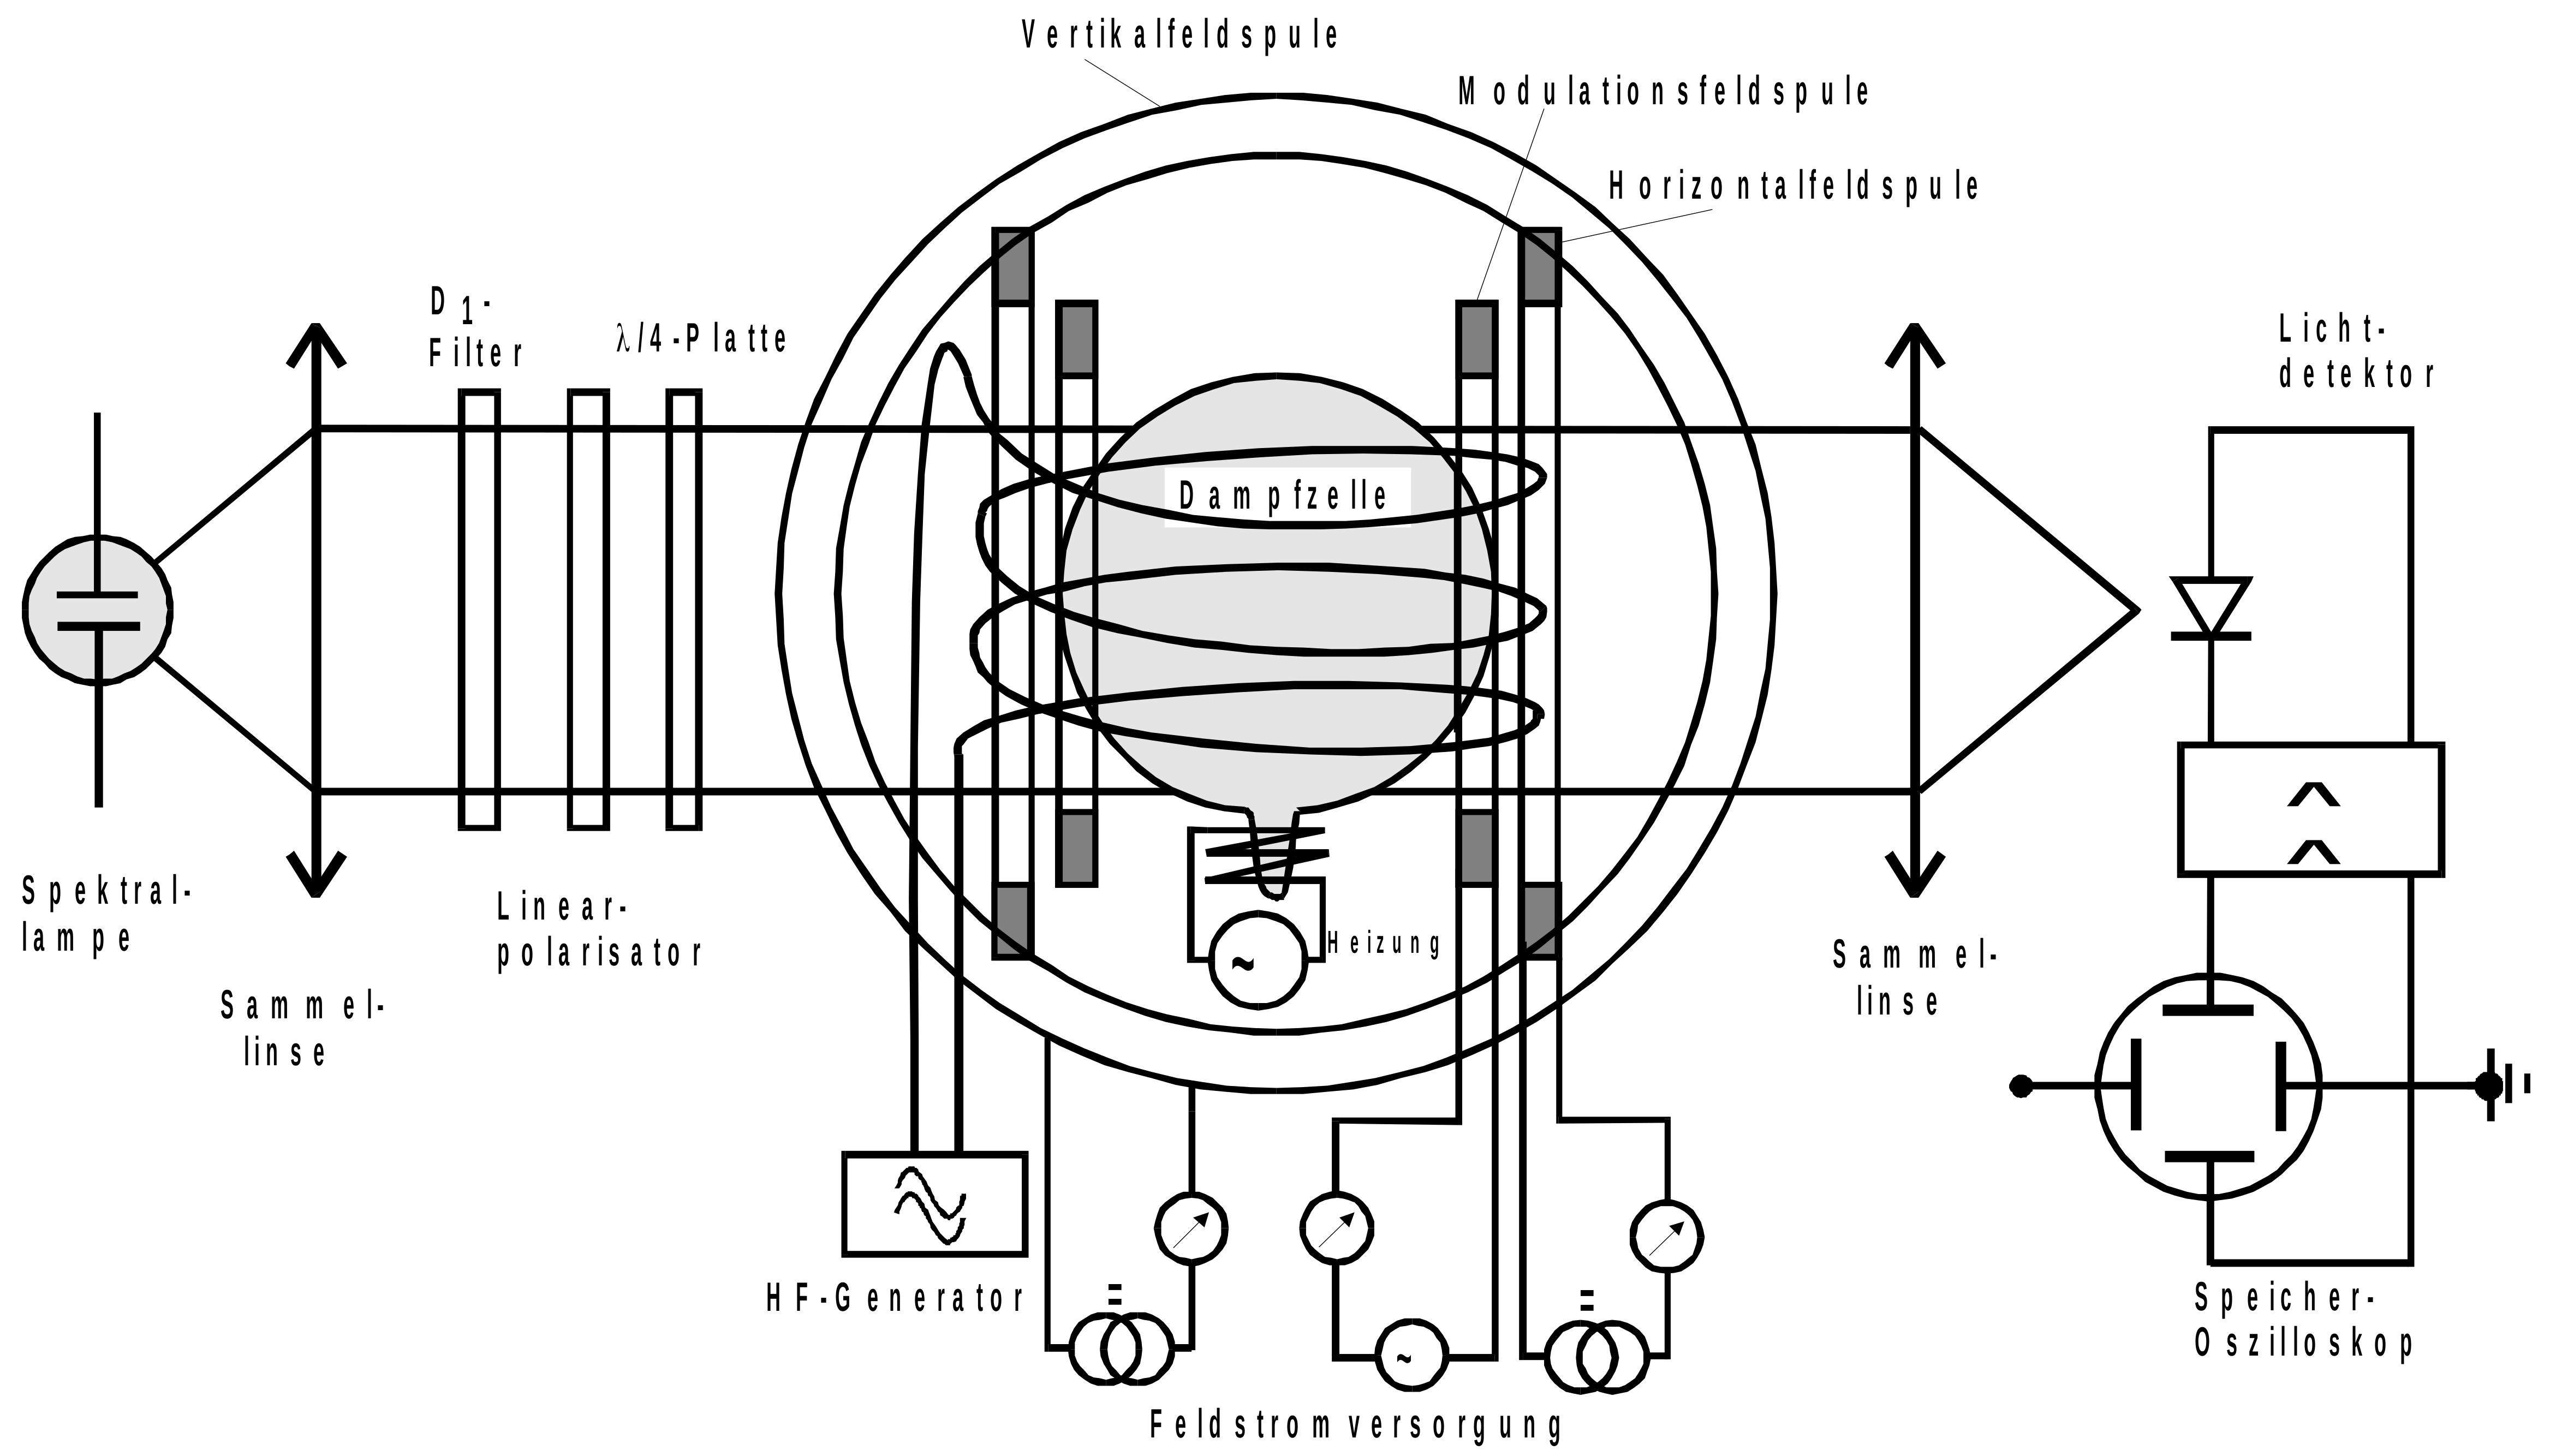
\includegraphics[width=0.8\textwidth]{images/aufbau.png}
    \caption{Schematischer Aufbau des Versuches \cite{anleitung}.}
    \label{fig:aufbau}
\end{figure}

Es stehen drei Helmholtzspulen zur Verfügung, um Magnetfelder anzulegen. Eine Horizontalfeldspule erzeugt ein
statisches Horizontalfeld, während die Sweep-Spule auf die Horizontalfeldspule aufgewickelt ist und ein
Sägezahnsignal liefert. Das RF-Feld wird mit einem externen Funktionsgenerator angesteuert.

\begin{table}
  \centering
  \caption{Daten der Spulen.}
  \label{tab:spulen}
  \begin{tabular}{c | S[table-format=3.0] S[table-format=2.3] S[table-format=1.1]}
    \toprule
    {Spule} & {Windungszahl $N$} & {Radius $r\;/\;\si{\centi\meter}$} & {Gainknopf} \\
    \midrule
    Sweep      &  11 & 16.39  & 0.3 \\
    Horizontal & 154 & 15.79  & 0.1 \\
    Vertikal   &  20 & 11.735 & 0.1 \\
    \bottomrule
  \end{tabular}
\end{table}
\section{Durchführung}

Zu Beginn des Versuchs wird der Strahlengang auf eine maximale Intensität eingestellt und die Apparatur abgedeckt,
um Streulicht von der Photozelle abzuhalten.
Das Prinzip der Messung ist, das Sweep-Feld auf den X-Eingang des Oszilloskops zu legen, sodass ein durchlaufender
Leuchtpunkt die Intensität in Abhängigkeit der Magnetfeldstärke zeigt.
Wenn nur das Sweep-Feld angelegt ist, wird ein breiter Dip bzw. Peak zu sehen sein (Nulldip in Abb.
\ref{fig:transparenz}), der dem Erdmagnetfeld zuzuordnen ist. Um seinen Effekt auf die Versuchsdurchführung zu
minimieren, wird das Vertikalfeld so eingestellt, dass der Dip möglichst schmal ist,
zusẗzlich wird der Tisch in Nord-Süd- Richtung orientiert.

Zur Bestimmung der RF-Feldstärke $B_m$, abhängig von der Frequenz des RF-Feldes, wird ein Frequenzgenerator mit
einem $\SI{4}{\volt}$ Sinus-Signal verwendet. Zu sehen sind zwei Dips für unterschiedliche $B_m$ aufgrund der
beiden Isotope des Rubidiums im Gasgemisch.
Für die Vermessung der Resonanzfrequenz gegen Magnetfeld wird die Frequenz von $\SI{100}{\kilo\hertz}$
bis $\SI{1}{\mega\hertz}$ durchfahren.
Zusätzlich wird bei einer Frequenz von $\SI{100}{\kilo\hertz}$ ein Bild des Signals dazu verwendet aus der
Tiefe der Dips das Isotopenverhältniss zu bestimmen.

%//////
Bei der Frequenz an den beiden Dips wird das Feld resonant eingestellt. Die RF-Spannung wird nun durch eine
Rechteckspannung auf dem \enquote{Input RF Modulation} mit einer Frequenz von $\SI{5}{\hertz}$ an- und ausgeschaltet.
Die RF-Frequenz selbst beträgt dabei $\SI{100}{\kilo\hertz}$. Dieses Signal wird auf Kanal 1 des Oszilloskops
gelegt, das in diesem Teil des Versuchs nicht im XY-Betrieb, sondern im YT-Betrieb läuft.
Aufgrund der Präzessionsbewegung des Spins ist eine exponentiell sättigende Transparenz für ein ausgeschaltetes
RF-Feld und eine Abschwingung für ein eingeschaltetes RF-Feld zu erkennen. Die Periodendauer dieser Oszillationen
wird für Amplituden von 2 bis $\SI{10}{\volt}$ für beide Isotope, also unterschiedliche Resonanzmagnetfeldstärken,
bestimmt.
